\definecolor{gray}{gray}{0.75}

\chapter{Data Collection and Processing}
In this section will be described on the process of collecting and processing data and analysis results are performed in accordance with the methodology described in the previous discussion.

\section{Data Collection}
At this stage, data are collected. Its to support kth nearest neighbour and route determination model. The data collected are as follows:

\subsection{Bandung road network map}
Data collected consist of Bandung administrative map and road network. Bandung road network map covers national road, provincial road, city road and some environmental road. However, the road network used in this study is only a network of arterial and collector class roads. To facilitate the processing of road network data, also required data vertex dividing the road network obtained based on the existing intersections.

\begin{figure}[H]
    \centering
    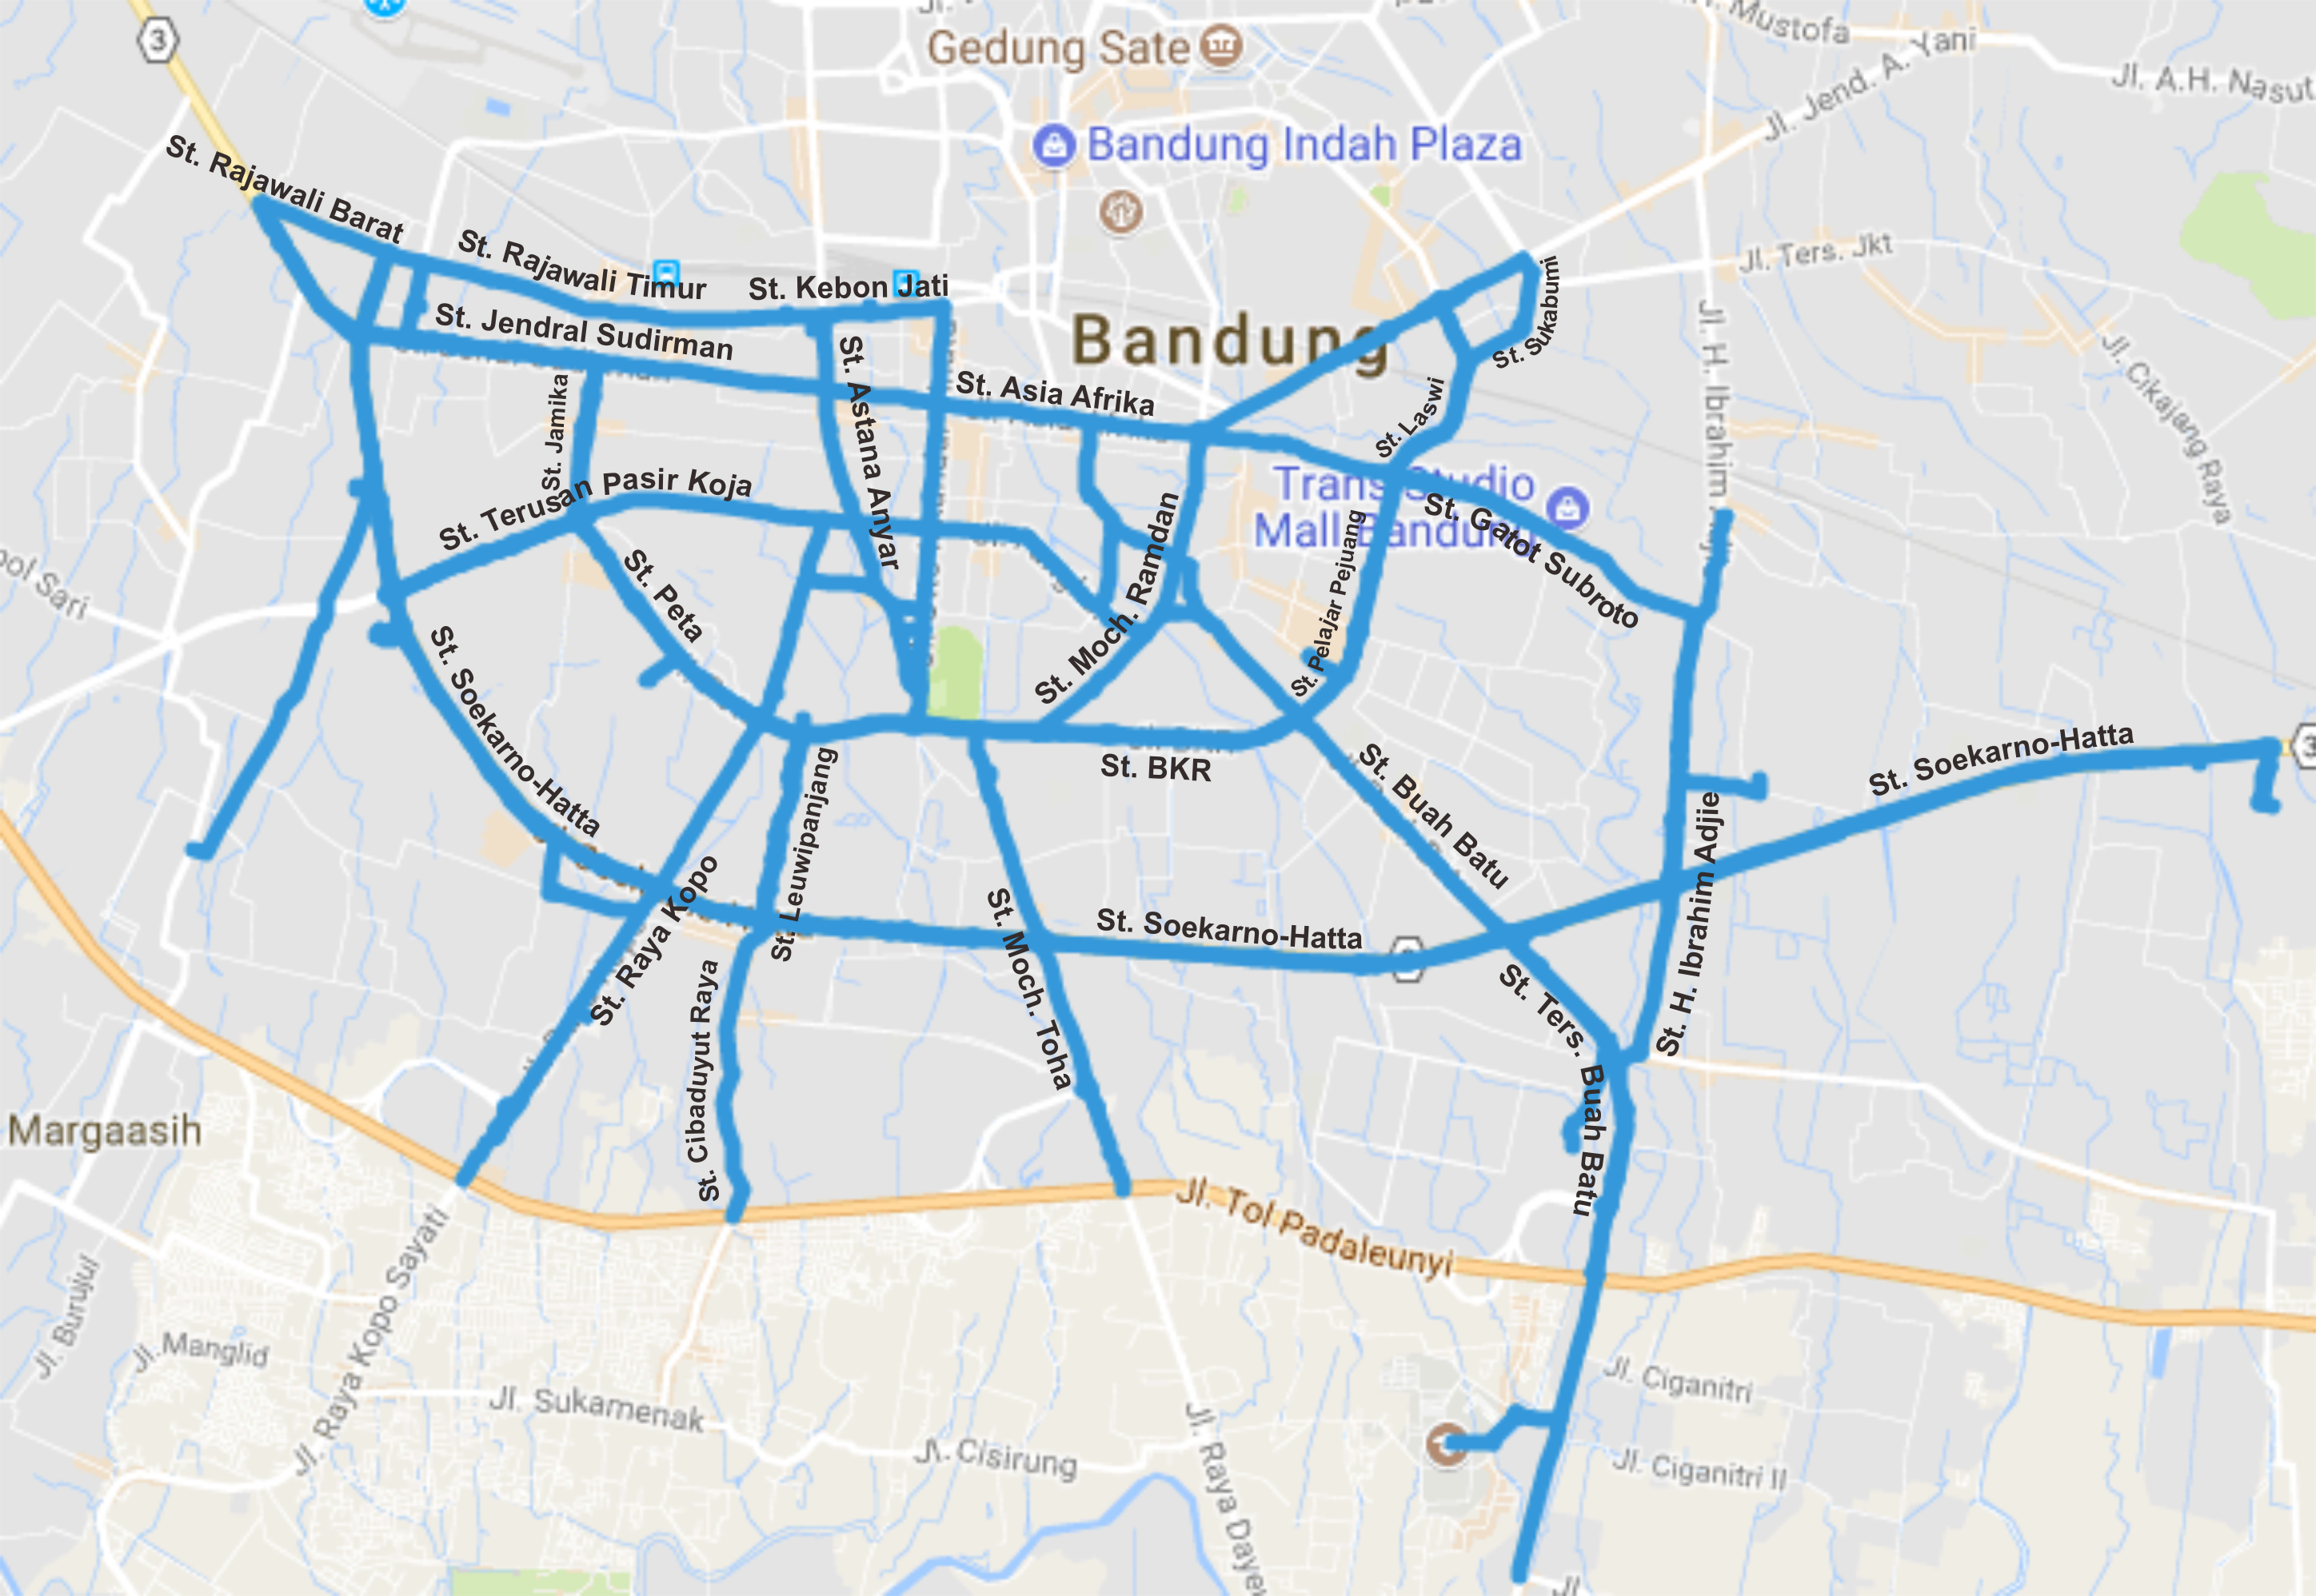
\includegraphics[scale=0.42]{data_coll1.png}
    \caption{Bandung administrative map}
    \label{fig:bandung_administrativ_map}
\end{figure}

\begin{table}[H] 
\centering
\begin{tabular}{|c|c|c|c|}
\hline
\rowcolor{gray}
\textbf{No} & \textbf{Name} & \textbf{Distance (km)} & \textbf{Status} \\
\hline
\multicolumn{2}{|l|}{\textit{Primary Artery Street}} &  & \\
\cline{1-4}
1. & \multicolumn{1}{|l|}{St. Jend. Sudirman} & 6,79 & National \\
\cline{1-4}
2. & \multicolumn{1}{|l|}{St. Asia Afrika} & 1,51 & National \\
\cline{1-4}
3. & \multicolumn{1}{|l|}{St. Soekarno-Hatta} & 18,46 & National \\

\cline{1-4}
\multicolumn{2}{|l|}{\textit{Secondary Artery Street}} &  & \\

\cline{1-4}
1. & \multicolumn{1}{|l|}{St. Peta} & 2,46 & Province \\
\cline{1-4}
2. & \multicolumn{1}{|l|}{St. BKR} & 2,30 & Province \\
\cline{1-4}
3. & \multicolumn{1}{|l|}{St. Pelajar Pejuang} & 1,56 & Province \\
\cline{1-4}
4. & \multicolumn{1}{|l|}{St. Laswi} & 1,17 & Province \\
\cline{1-4}
5. & \multicolumn{1}{|l|}{St. Gatot Subroto} & 1,68 & Province \\
\cline{1-4}
6. & \multicolumn{1}{|l|}{St. Jamika} & 0,91 & City \\
\cline{1-4}
7. & \multicolumn{1}{|l|}{St. Sukabumi} & 0,64 & City \\
\hline
\end{tabular}
\caption{Artery Road Data}
\label{table:street_data1}
\end{table}

\begin{table}[H] 
\centering
\begin{tabular}{|c|c|c|c|}
\hline
\rowcolor{gray}
\textbf{No} & \textbf{Name} & \textbf{Distance (km)} & \textbf{Status} \\
\hline
\multicolumn{2}{|l|}{\textit{Primary Collector Street}} &  & \\
\cline{1-4}
1. & \multicolumn{1}{|l|}{St. Pasir Koja} & 0,13 & Province \\
\cline{1-4}
2. & \multicolumn{1}{|l|}{St. Ters. Pasir Koja} & 2,72 & Province \\
\cline{1-4}
3. & \multicolumn{1}{|l|}{St. Raya Kopo} & 2,96 & Province \\
\cline{1-4}
4. & \multicolumn{1}{|l|}{St. Buah Batu} & 0,99 & Province \\
\cline{1-4}
5. & \multicolumn{1}{|l|}{St. Ters. Buah Batu} & 1,06 & Province \\
\cline{1-4}
6. & \multicolumn{1}{|l|}{St. H. Ibrahim Adjie} & 1,16 & Province \\
\cline{1-4}
7. & \multicolumn{1}{|l|}{St. Moch. Toha} & 3,47 & Province \\
\cline{1-4}
8. & \multicolumn{1}{|l|}{St. Leuwipanjang} & 1,08 & Province \\
\cline{1-4}
9. & \multicolumn{1}{|l|}{St. Cibaduyut Raya} & 1,72 & Province \\
\cline{1-4}
10. & \multicolumn{1}{|l|}{St. Astana Anyar} & 0,76 & City \\
\cline{1-4}
11. & \multicolumn{1}{|l|}{St. Moch. Ramdan} & 0,94 & City \\
\cline{1-4}
\multicolumn{2}{|l|}{\textit{Secondary Collector Street}} &  & \\
\cline{1-4}
1. & \multicolumn{1}{|l|}{St. Rajawali Barat} & 1,02 & Nasional \\
\cline{1-4}
2. & \multicolumn{1}{|l|}{St. Rajawali Timur} & 1,54 & Nasional \\
\cline{1-4}
3. & \multicolumn{1}{|l|}{St. Kebonjati} & 1,40 & Provinsi \\
\hline
\end{tabular}
\caption{Collector Road Data}
\label{table:street_data1}
\end{table}

\pagebreak

\subsection{Ambulance Location in Bandung}
The location point of the emergency unit in Bandung was obtained through field observation. Data coordinates the location of this emergency unit obtained from the Bandung data portal. Ambulance Location based on the coordinate point shown in figure \ref{fig:ambulance_location}
\begin{figure}[H]
    \centering
    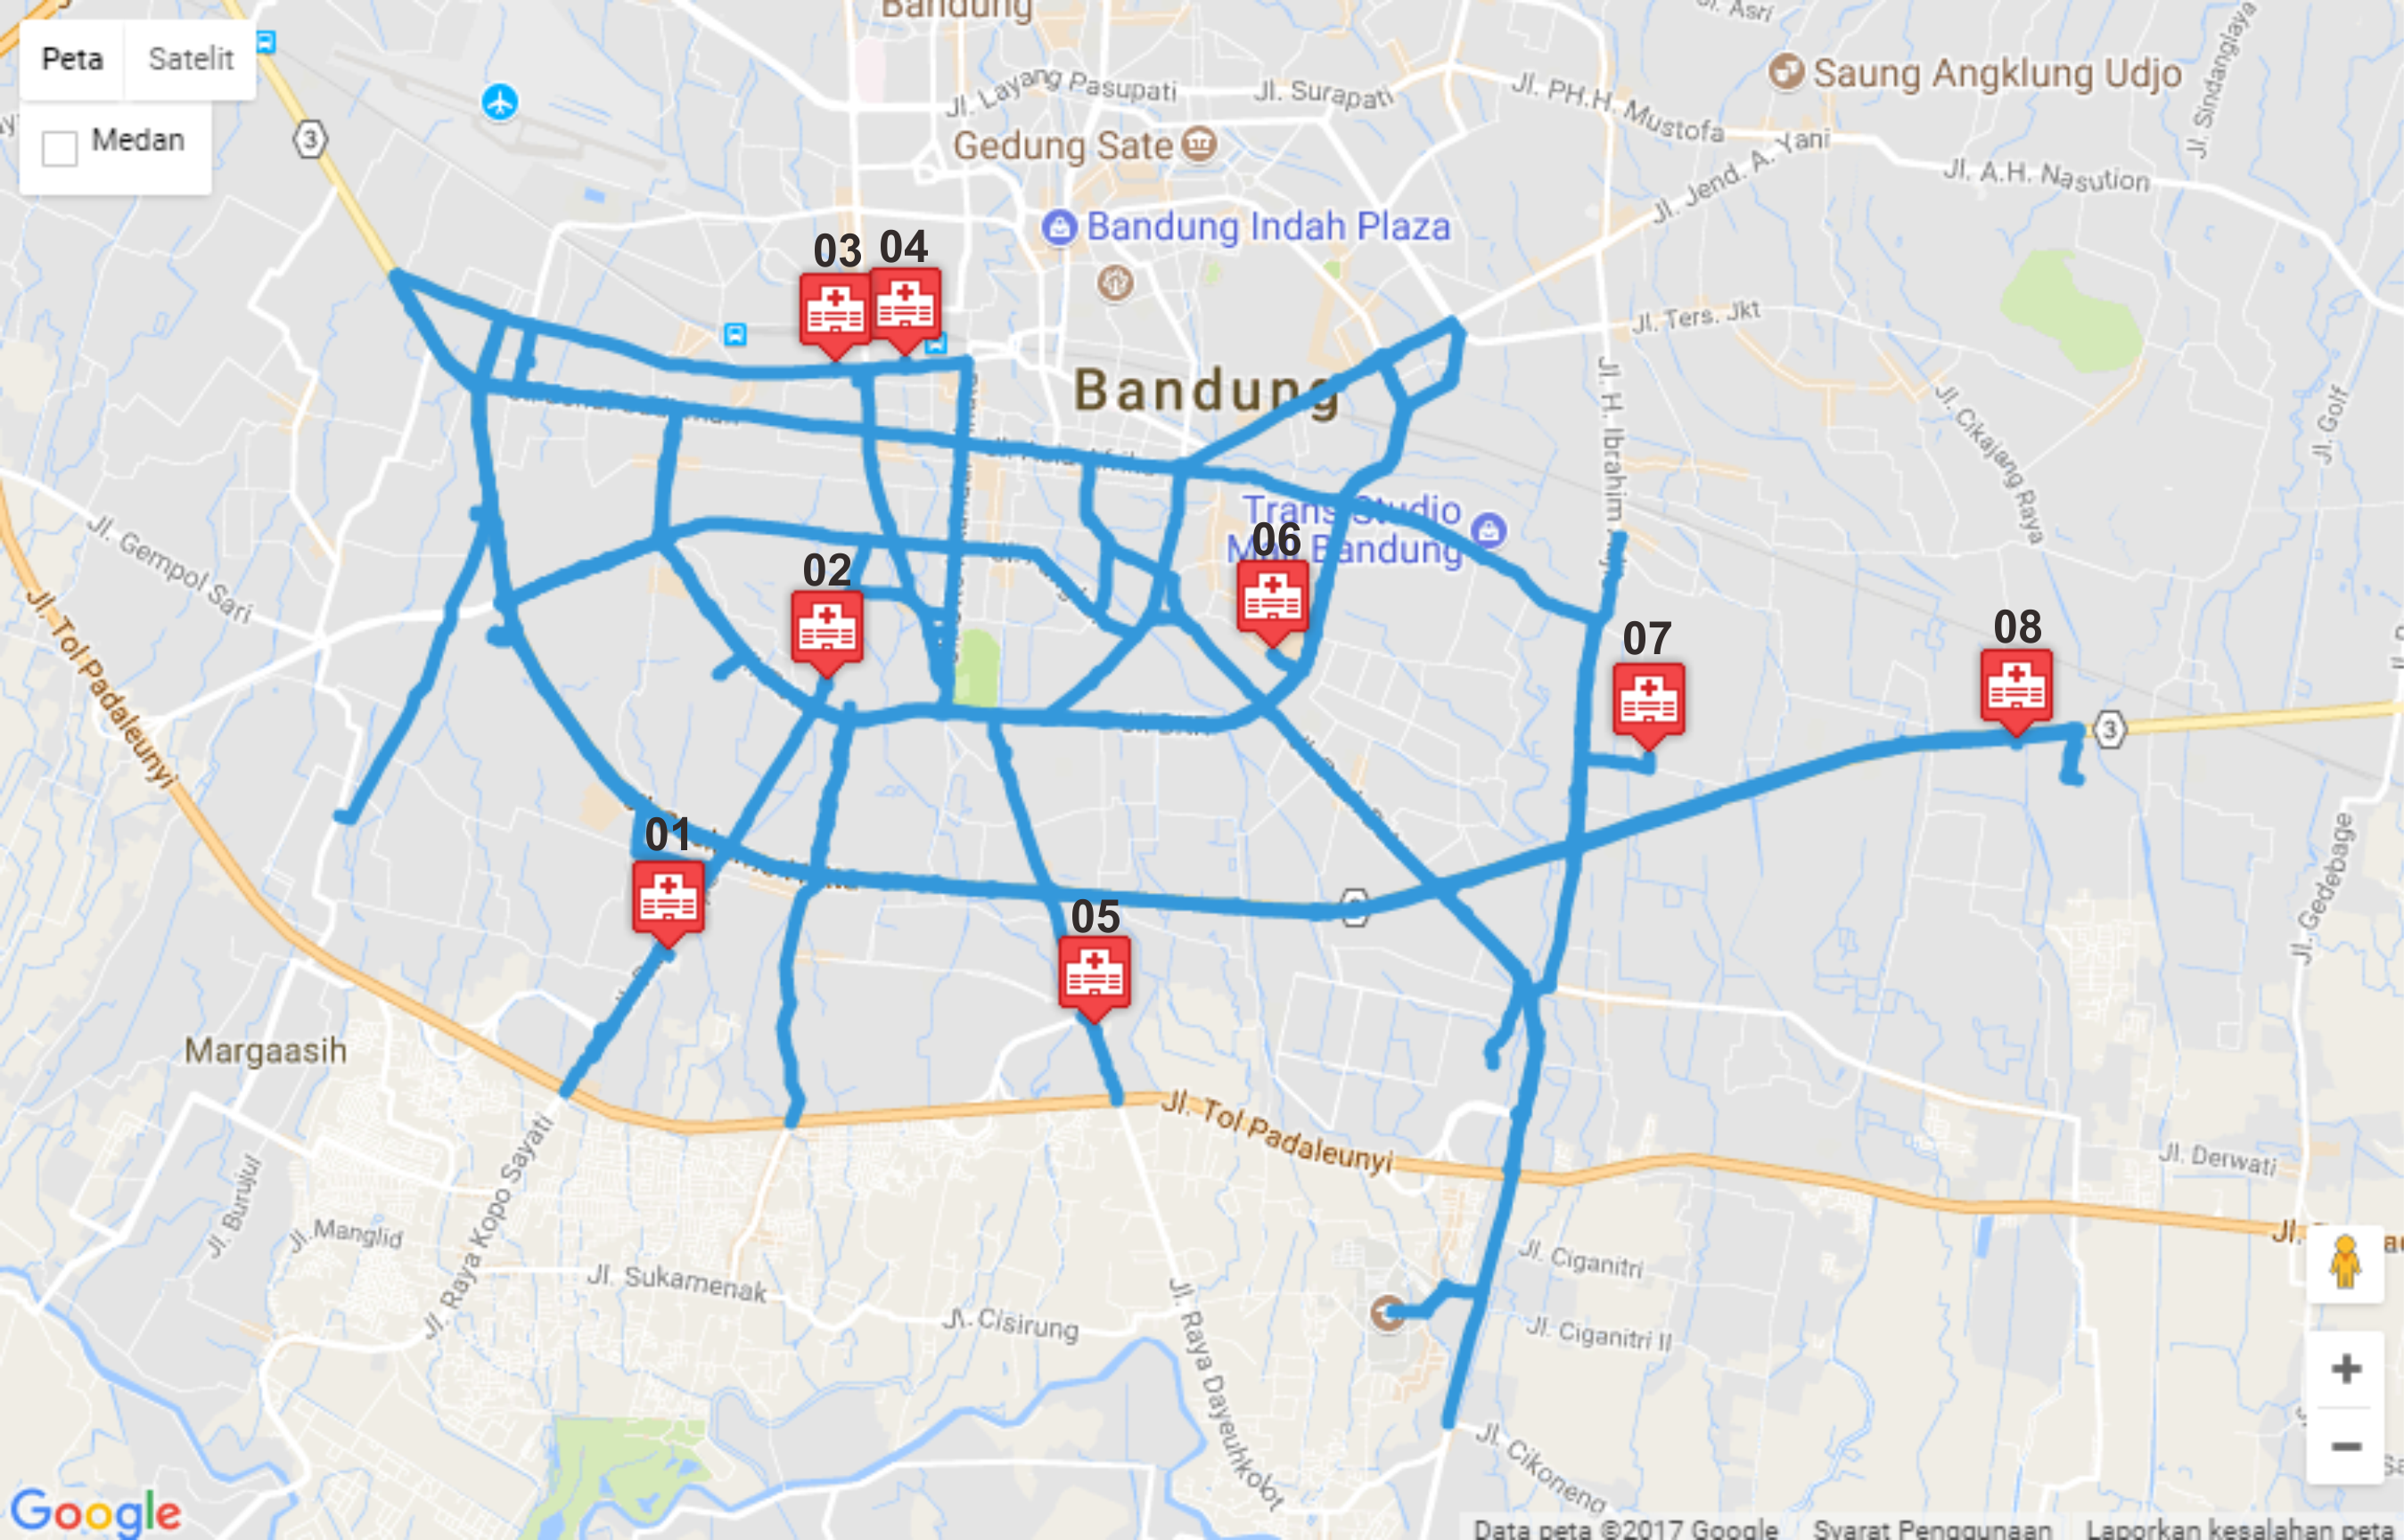
\includegraphics[scale=0.6]{data_coll2.png}
    \caption{Ambulance location in Bandung}
    \label{fig:ambulance_location}
\end{figure}

The symbols, captions, and coordinate points of figure \ref{fig:ambulance_location} are described in the table \ref{table:ambulance_data} below:

\begin{table}[H] 
\centering
\begin{tabular}{|c|c|c|c|c|}
\hline
\rowcolor{gray}
\textbf{No} & \textbf{Id} & \textbf{Name} & \textbf{Latitude} & \textbf{Longitude} \\
\hline
1. & AMB001 & \multicolumn{1}{|l|}{RSU Santosa Kopo} & -6.952198 & 107.586060 \\
\cline{1-5}
2. & AMB002 & \multicolumn{1}{|l|}{RSU Immanuel} & -6.935604 & 107.595856 \\
\cline{1-5}
3. & AMB003 & \multicolumn{1}{|l|}{RSU Kebonjati} & -6.916139 & 107.596306 \\
\cline{1-5}
4. & AMB004 & \multicolumn{1}{|l|}{RSU Santosa Bandung Central} & -6.915867 & 107.600533 \\
\cline{1-5}
5. & AMB005 & \multicolumn{1}{|l|}{RSU Sartika Asih} & -6.956771 & 107.612312 \\
\cline{1-5}
6. & AMB006 & \multicolumn{1}{|l|}{RSU Muhammadiyah} & -6.933718 & 107.623299 \\
\cline{1-5}
7. & AMB007 & \multicolumn{1}{|l|}{RSU KCK Pindad} & -6.939983 & 107.646523  \\
\cline{1-5}
8. & AMB008 & \multicolumn{1}{|l|}{RSU Al-Islam} & -6.939277 & 107.6691134 \\
\hline
\end{tabular}
\caption{Ambulance Data}
\label{table:ambulance_data}
\end{table}

\subsection{Police Location in Bandung}
The location point of the emergency unit in Bandung was obtained through field observation. Data coordinates the location of this emergency unit obtained from the Bandung data portal. Police Location based on the coordinate point shown in figure \ref{fig:police_location}

\begin{figure}[H]
    \centering
    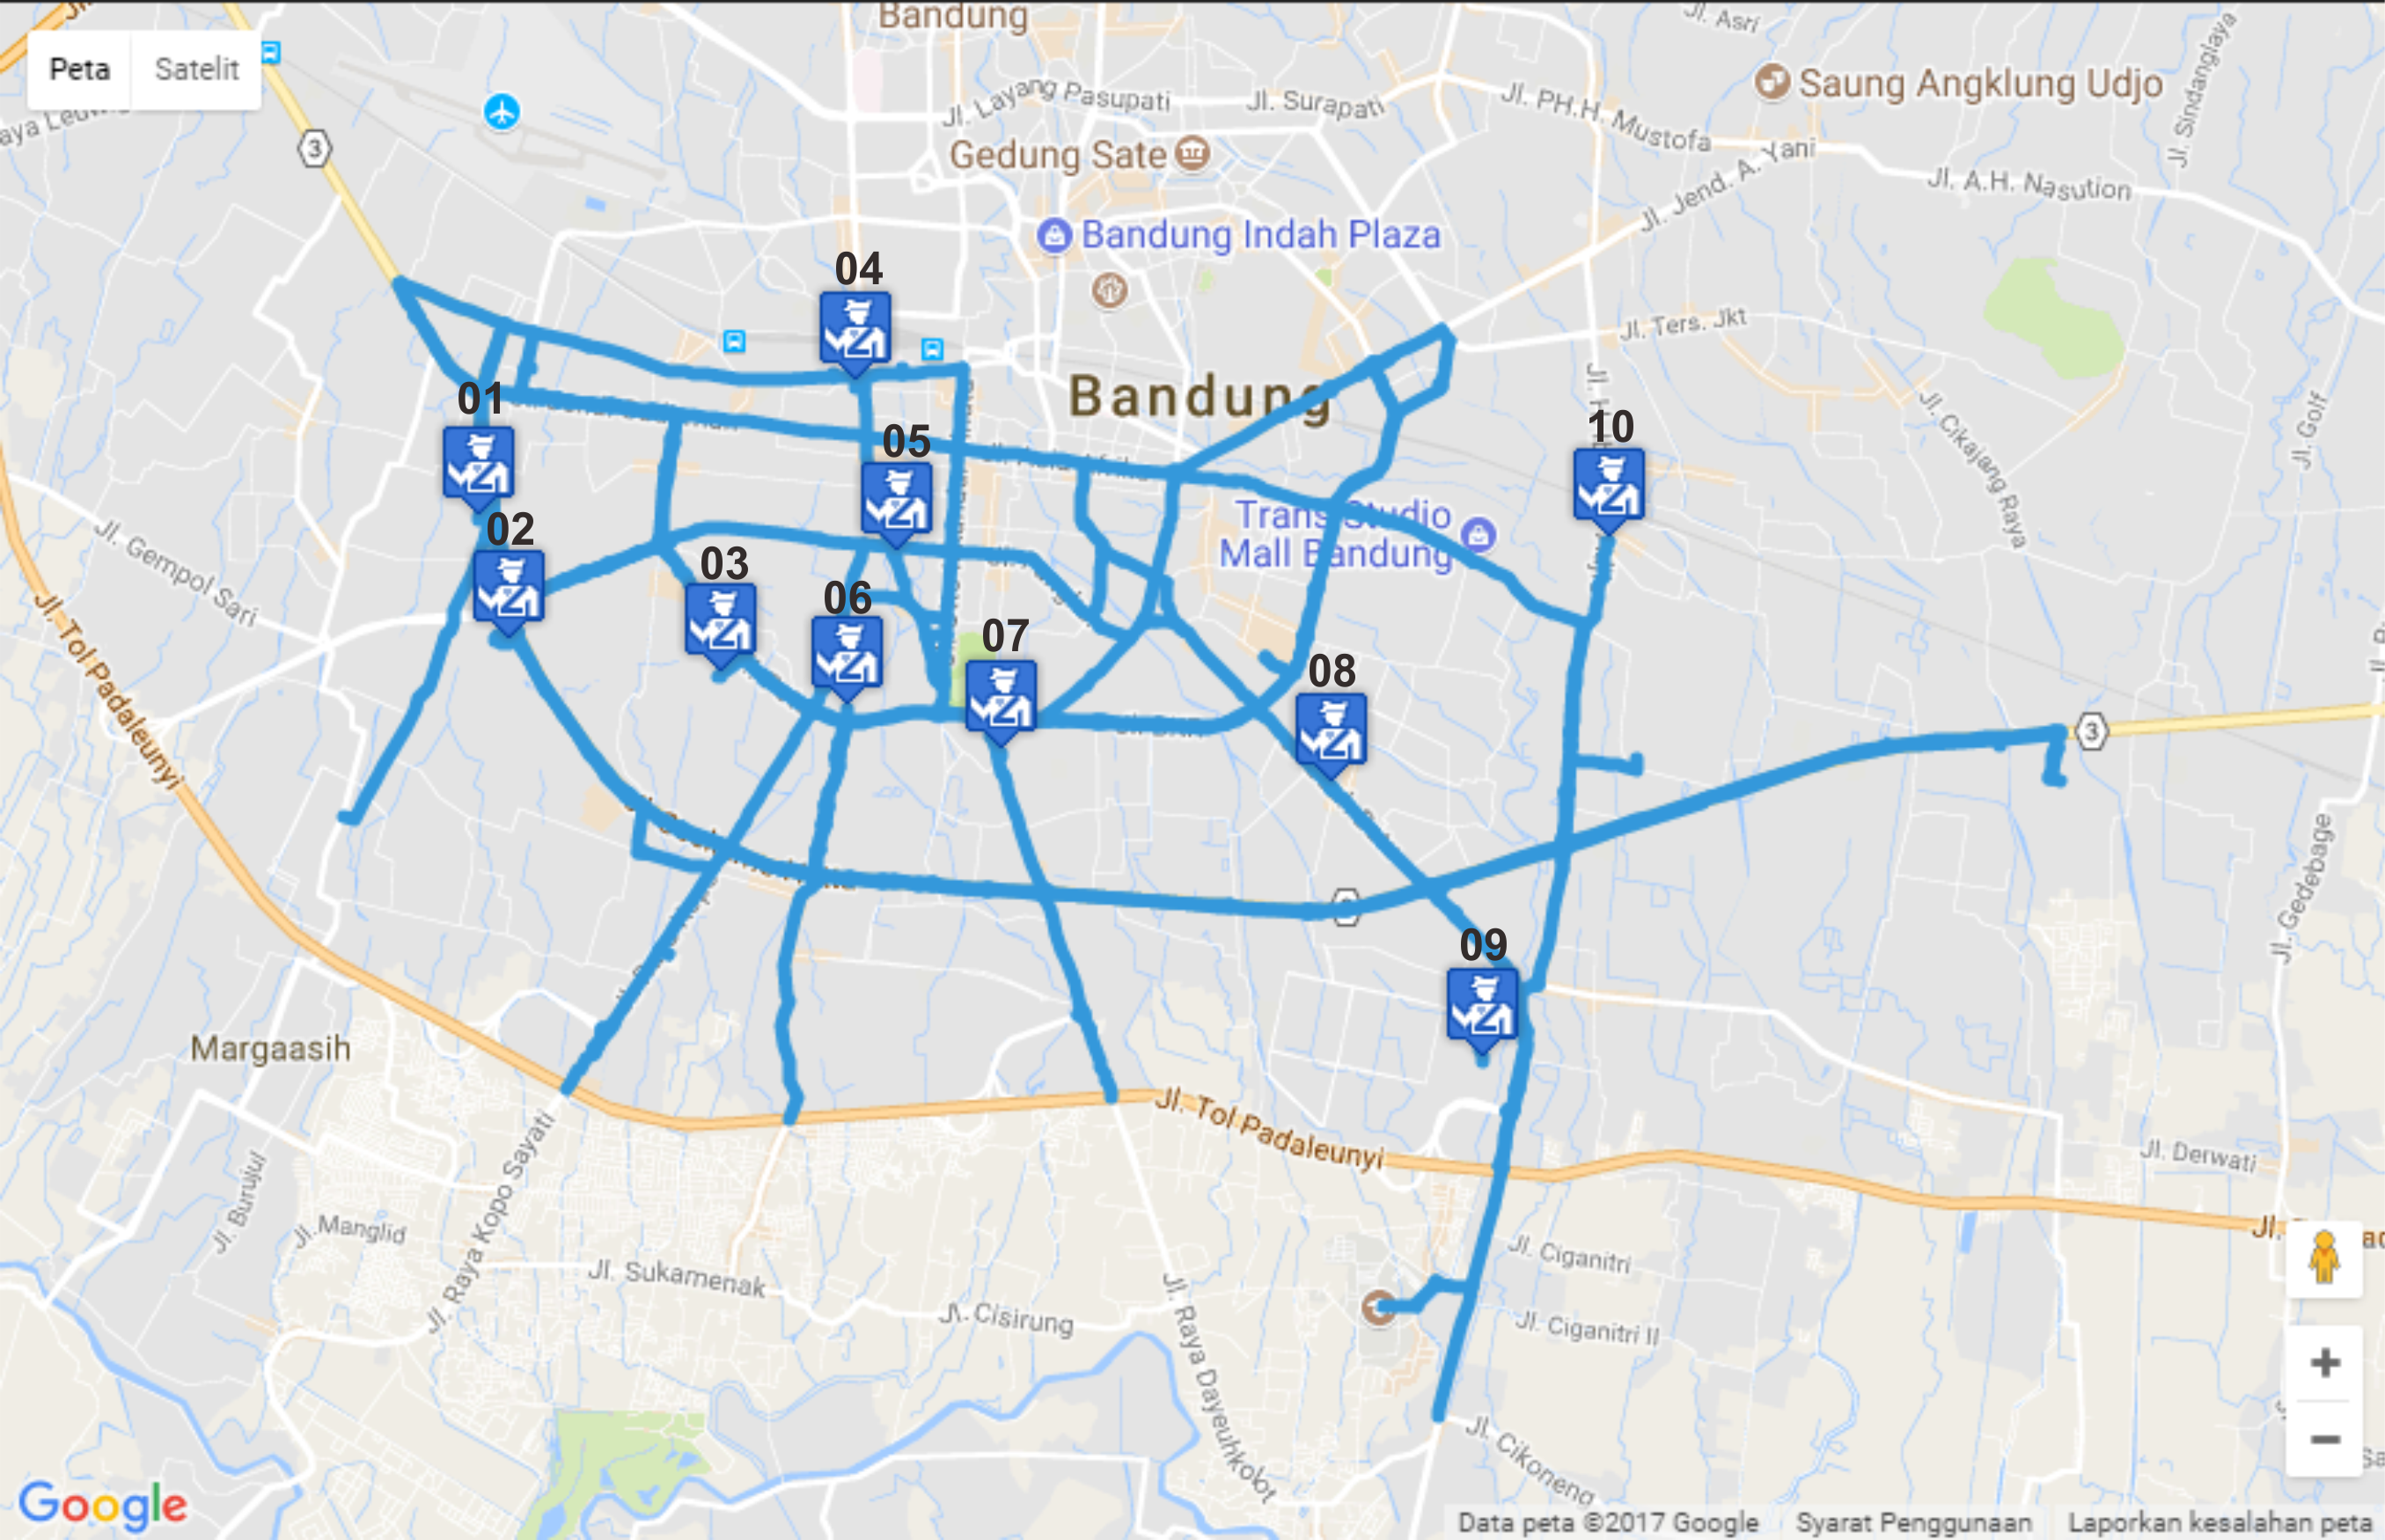
\includegraphics[scale=0.6]{data_coll3.png}
    \caption{Police location in Bandung}
    \label{fig:police_location}
\end{figure}

The symbols, captions, and coordinate points of figure \ref{fig:police_location} are described in the table \ref{table:police_data} below:

\begin{table}[H] 
\centering
\begin{tabular}{|c|c|c|c|c|}
\hline
\rowcolor{gray}
\textbf{No} & \textbf{Id} & \textbf{Name} & \textbf{Latitude} & \textbf{Longitude} \\
  \hline
1. & POL001 & \multicolumn{1}{|l|}{Polsek Bandung Kulon} & -6.925269 & 107.574158 \\
  \cline{1-5}
2. & POL002 & \multicolumn{1}{|l|}{Polsek Babakan Ciparay} & -6.932978 & 107.575981 \\
  \cline{1-5}
3. & POL003 & \multicolumn{1}{|l|}{Polsek Bojongloa Kaler} & -6.935009 & 107.589287 \\
  \cline{1-5}
4. & POL004 & \multicolumn{1}{|l|}{Polsek Andir} & -6.916926 & 107.597664 \\
  \cline{1-5}
5. & POL005 & \multicolumn{1}{|l|}{Polsek Astana Anyar} & -6.927466 & 107.600204 \\
  \cline{1-5}
6. & POL006 & \multicolumn{1}{|l|}{Polsek Bojongloa Kidul} & -6.937067 & 107.597115 \\
   \cline{1-5}
7. & POL007 & \multicolumn{1}{|l|}{Polsek Regol} & -6.939767 & 107.606819 \\
  \cline{1-5}
8. & POL008 & \multicolumn{1}{|l|}{Polsek Lengkong} & -6.941817 & 107.627449 \\
   \cline{1-5}
9. & POL009 & \multicolumn{1}{|l|}{Polsek Bandung Kidul} & -6.958753 & 107.636917  \\
   \cline{1-5}
10. & POL010 & \multicolumn{1}{|l|}{Polsek Kiaracondong} & -6.926602 & 107.644714 \\
  \hline
\end{tabular}
\caption{Police Data}
\label{table:police_data}
\end{table}


\subsection{Fire Brigade in Bandung}
The location point of the emergency unit in Bandung was obtained through field observation. Data coordinates the location of this emergency unit obtained from the Bandung data portal. Police Location based on the coordinate point shown in figure \ref{fig:fire_brigade_location}

\begin{figure}[H]
    \centering
    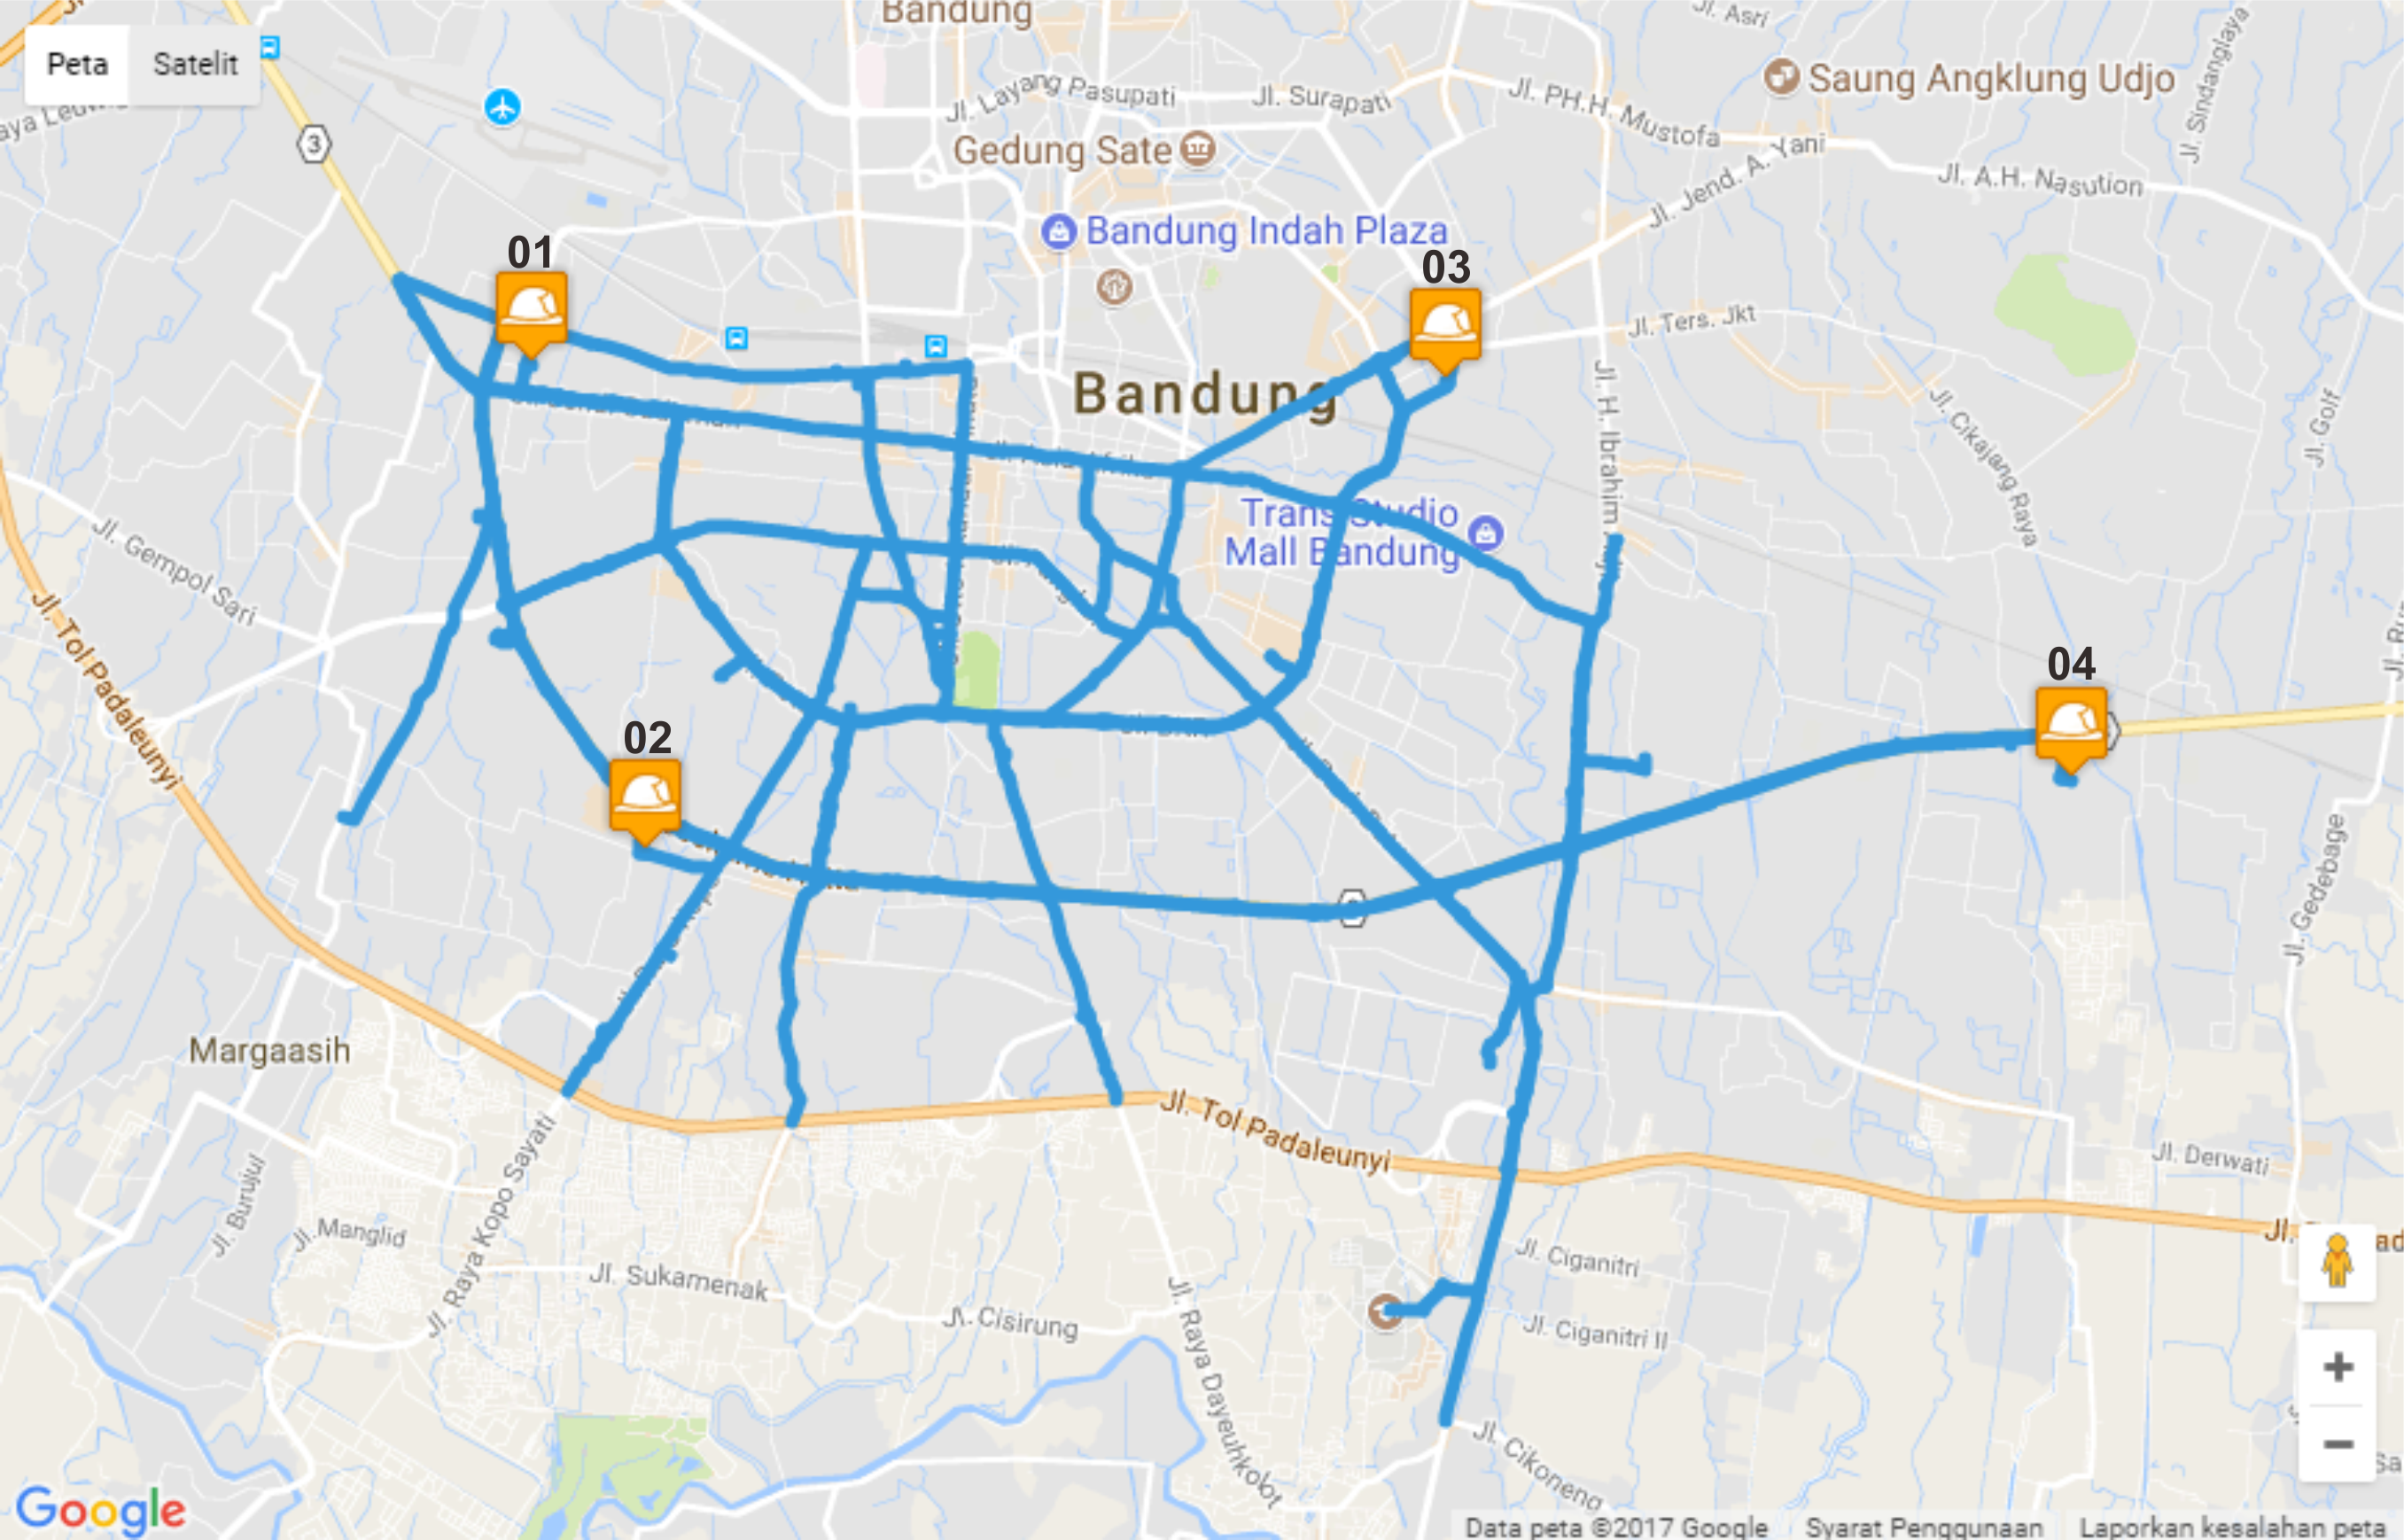
\includegraphics[scale=0.6]{data_coll4.png}
    \caption{Fire Brigade location in Bandung}
    \label{fig:fire_brigade_location}
\end{figure}

The symbols, captions, and coordinate points of figure \ref{fig:fire_brigade_location} are described in the table \ref{table:fire_brigade_data} below:

\begin{table}[H] 
\centering
\begin{tabular}{|c|c|c|c|c|}
\hline
\rowcolor{gray}
\textbf{No} & \textbf{Id} & \textbf{Name} & \textbf{Latitude} & \textbf{Longitude} \\
\hline
1. & FBR001 & \multicolumn{1}{|l|}{UPT Damkar Wilayah Barat} & -6.915912 & 107.577354 \\
\cline{1-5}
2. & FBR002 & \multicolumn{1}{|l|}{UPT Damkar Wilayah Selatan} & -6.945922 & 107.584412  \\
\cline{1-5}
3. & FBR003 & \multicolumn{1}{|l|}{Dinas Kebakaran Kota Bandung} & -6.916825 & 107.634109 \\
\cline{1-5}
4. & FBR004 & \multicolumn{1}{|l|}{UPT Damkar Wilayah Timur} & -6.941342 & 107.672874 \\
\hline
\end{tabular}
\caption{Fire Brigade Data}
\label{table:fire_brigade_data}
\end{table}

\pagebreak

\section{Data Processing}
Data processing is done to get the nearest generator from query point and calculate optimal route from the generator to the query point based on the shortest route. In this case, a nearby generator search is made up of units such as police, ambulance, and fire brigade. Then calculate optimal route from selected units to the query point which is the scene of the accident.

\subsection{Constructing Network Voronoi Diagram}
This step intended to divides road network into subnetworks which are act as a coverage area for an emergency unit. These coverage area always returns its generator for nearest emergency unit. This step consists two following process which are border point determination and nearest emergency unit classification.

\subsubsection{- Determining Border Point}
This step intended to determine the border point between adjacent units by expanding each unit so that each unit has at least been a starting point. Expansion is done using queue which sorted by minimum distance. The following example presents an example of data processing to get the border points of the RSU Al-Islam to its neighbor generator.

\begin{figure}[H]
    \centering
    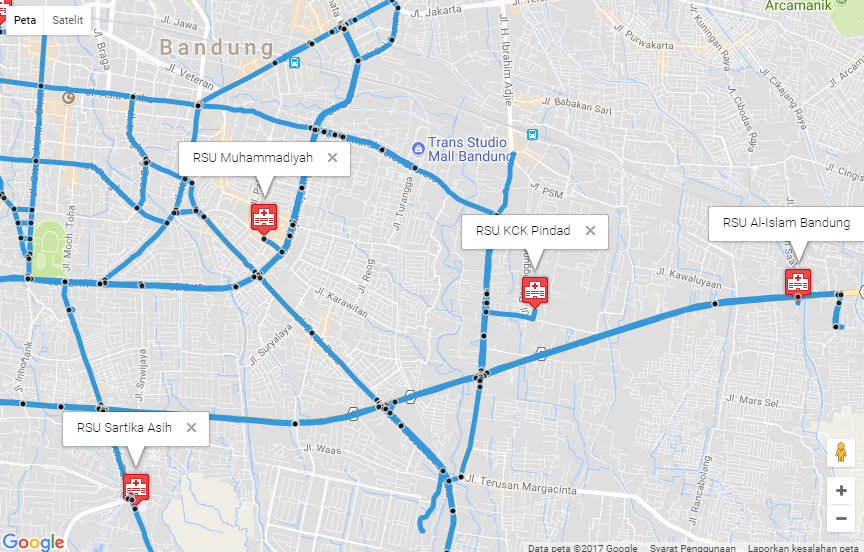
\includegraphics[scale=0.53]{data_proc_1_1.png}
    \caption{RSU Al-Islam Map}
    \label{fig:rsu_al-islam_map}
\end{figure}

\begin{table}[H]
\centering
\begin{tabular}{lll}
Id Vertex & = & 20           \\
Name      & = & RSU Al-Islam \\
Unit Type & = & Ambulance   
\end{tabular}
\end{table}

Vertex 20 inserted into the queue and act as $v_{selected}$. For each vertex that shares same edge with vertex 20 will be checked its type. So expanding process when meets another generator RSU KCK Pindad is shown in \ref{fig:alur_expand} below:

\begin{figure}[H]
    \centering
    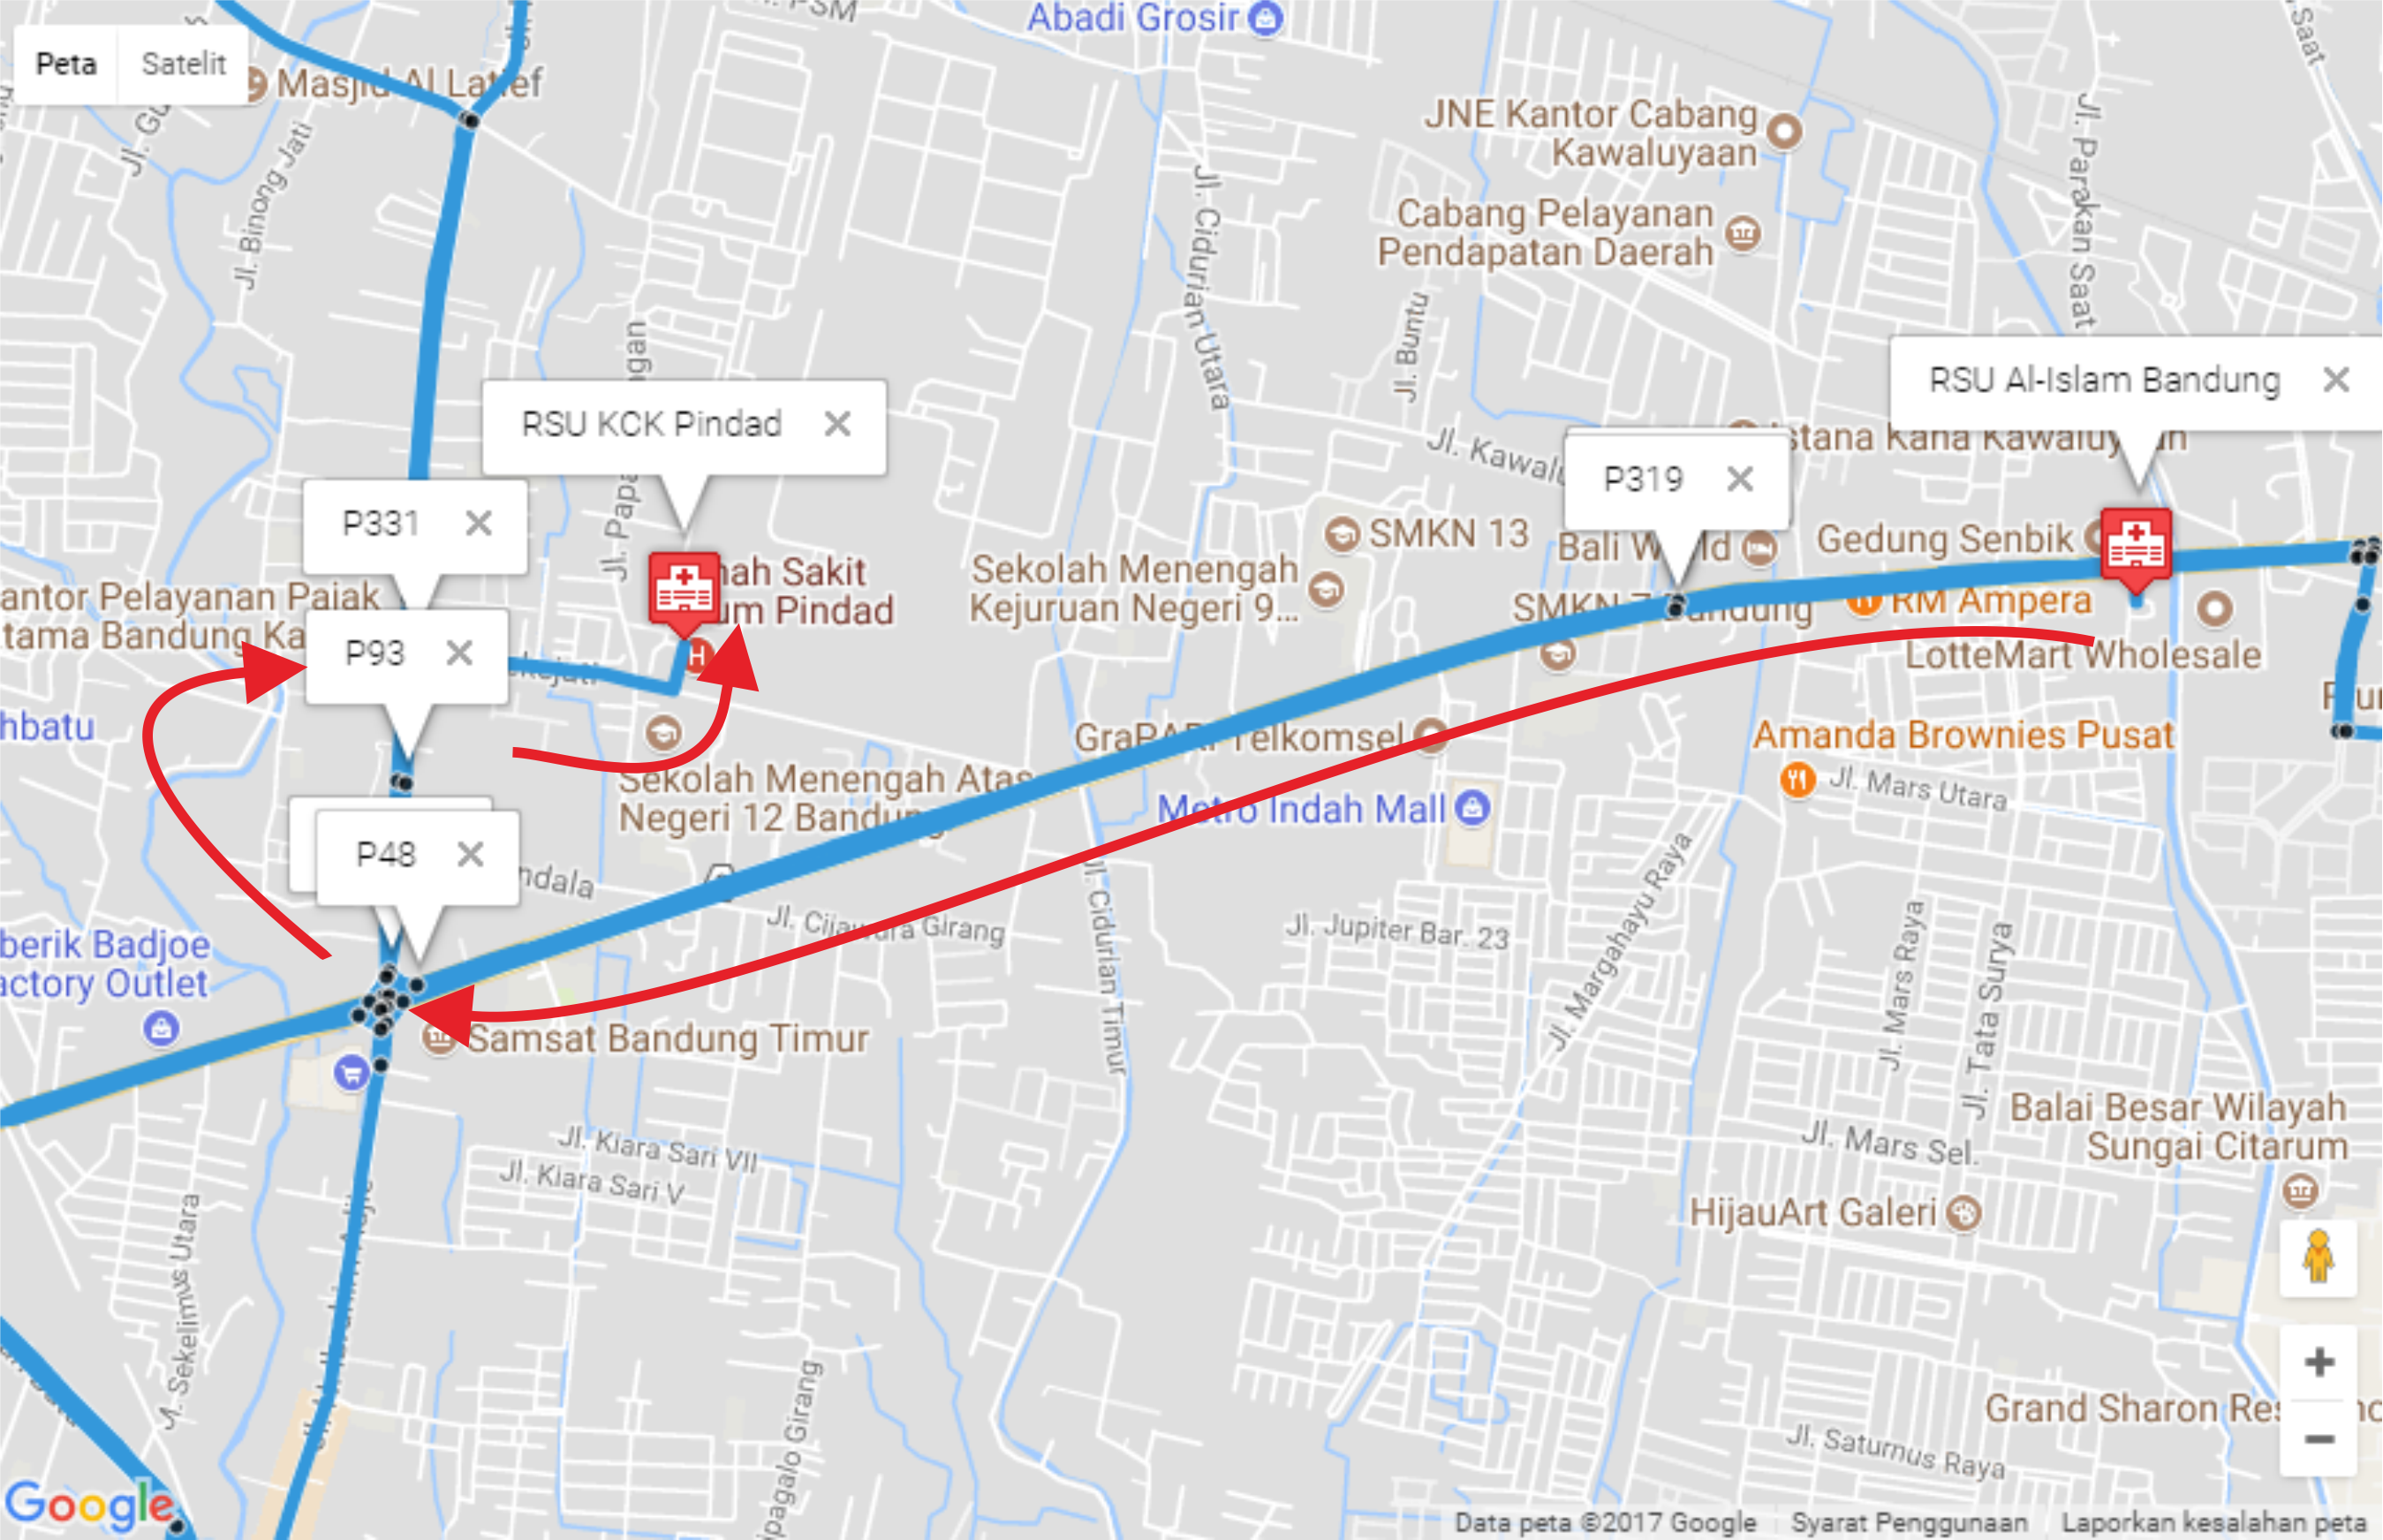
\includegraphics[scale=0.55]{data_proc_1_2.png}
    \caption{Expansion Flow of RSU Al-Islam Hospital to RSU KCK Pindad}
    \label{fig:alur_expand}
\end{figure}

\begin{table}[H]
\begin{tabular}{lll}
Path & = & 322-323-318-48-49-93-331-330 \\
Total Distance & = & 4.2903026796279 km\\
\end{tabular}
\end{table}

From the path data, border points can be obtained by determine middle distance from RSU Al-Islam and RSU KCK Pindad as follows:

\begin{table}[H]
\begin{tabular}{lll}
Mid Distance & = & 2,14515 km \\
Subdistance & = & 0,048559089918396 km\\
Edge Selected & = & N48N318\\
 & &\\
Edge Point 1 Id  & = & N48N318-08\\
Edge Point 1 Latitude & = & -6.943101\\
Edge Point 1 Longitude & = & 107.648819\\
 & &\\
Edge Point 2 Id  & = & N48N318-07\\
Edge Point 2 Id  & = & -6.942309\\
Edge Point 2 Id  & = & 107.651390\\
\end{tabular}
\end{table}

After that, calculation of the border point needs to determine its exact coordinates.

\begin{table}[H] 
\begin{tabular}{lll}
$fp$ & = & $subDistance / distance_{edgepoint2}$ \\
$fp$ & = & $0.048559089918396 / 0.299476$ \\
$fp$ & = & $0.16214684955855$ \\
\end{tabular}
\end{table}

\begin{table}[H] 
\begin{tabular}{lll}
$Lat_{mid}$ & = & $(Lat_{edgepoint2} \times (1-fp)) + (Lat_{edgepoint1} \times fp)$ \\
$Lat_{mid}$ & = & $(-6.943101 \times (1-0.16214)) + (-6.942309 \times 0.16214)$ \\
$Lat_{mid}$ & = & $-6.9424374203049$ \\
 & & \\
$Long_{mid}$ & = & $(Long_{edgepoint2} \times (1-fp)) + (Long_{edgepoint1} \times fp)$ \\
$Long_{mid}$ & = & $(107.651390 \times (1-0.16214)) + (107.648819 \times 0.16214)$ \\
$Long_{mid}$ & = & $107.6509731204$ \\
\end{tabular}
\end{table}

So the border point coordinates between RSU Al-Islam and RSU KCK Pindad is shown in \ref{fig:rsu_border_point} below:

\begin{figure}[H]
    \centering
    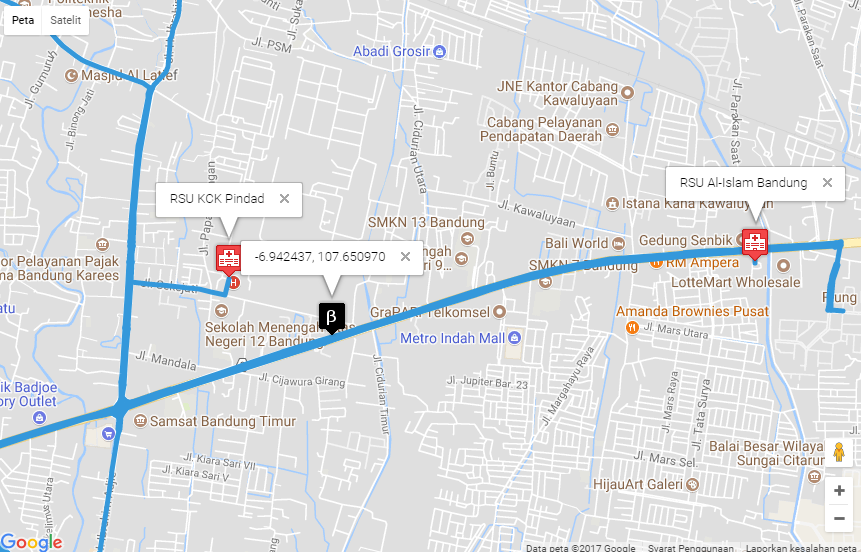
\includegraphics[scale=0.55]{data_proc_1_3.png}
    \caption{Border Point 441 Location}
    \label{fig:rsu_border_point}
\end{figure}

\begin{table}[H]
\centering
\begin{tabular}{lcl}
Id Vertex & =                     & 441              \\
Latitude  & =                     & -6.9424374203049 \\
Longitude & \multicolumn{1}{l}{=} & 107.65097312045 
\end{tabular}
\end{table}

\pagebreak

\subsubsection{- Classifying Nearest Emergency Unit}
The construction of network voronoi diagram is done by classifying nearest generator of all vertices. So network voronoi diagram will generating the coverage area of each generator which always returns its generator for nearest emergency unit. The following example shows the classification of the nearest ambulance generator of a vertex. Data attributes to be classified are as follows:

\begin{figure}[H]
    \centering
    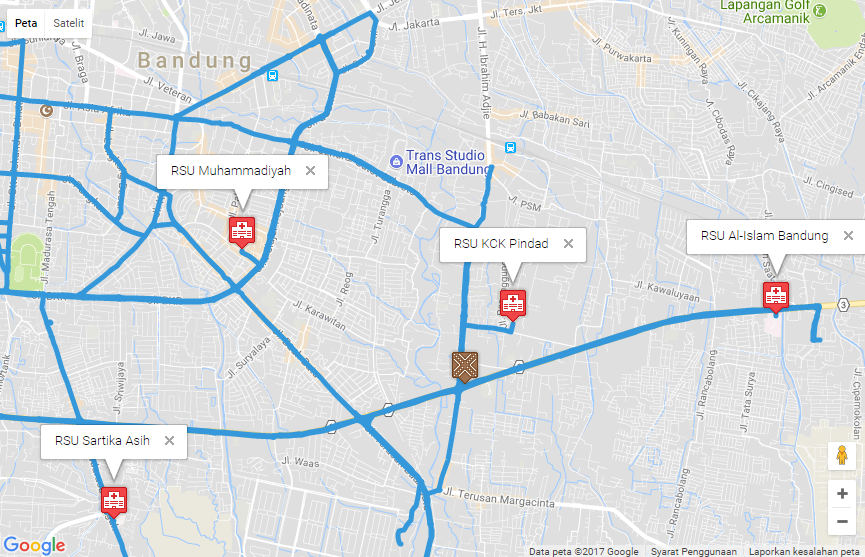
\includegraphics[scale=0.55]{data_proc_nvd_construction_1.png}
    \caption{Vertex 48 Location}
    \label{fig:rsu_border_point}
\end{figure}

\begin{table}[H]
\centering
\begin{tabular}{lll}
Id Vertex & = & 48 \\
Latitude & = & -6.945233 \\
Longitude & = & 107.642380 \\
\end{tabular}
\end{table}

Initialization queue is done first by entering data of each ambulance unit. Queue is sorted by the minimum distance to the emergency location (QP). After the insertion, the contents of queue are shown as follows.

\begin{table}[H] 
\centering
\begin{tabular}{|c|c|l|c|}
\hline
\textbf{No} & \textbf{$v_{id}$} & \textbf{$v_{data}$} & \textbf{$v_{distance}$}\\
\hline
1 &  322 & 322 (RSU Al-Islam Bandung) & 0\\
\hline
2 & 322 & 324 (RSU Kebonjati) & 0\\
\hline
3 & 328 & 328 (RSU Santosa Bandung Central) & 0\\
\hline
4 & 330 & 330 (RSU KCK Pindad) & 0\\
\hline
5 & 332 & 332 (RSU Sartika Asih) & 0\\
\hline
6 & 334 & 334 (RSU Santosa Bandung Kopo) & 0\\
\hline
7 & 336 & 336 (RSU Immanuel) & 0\\
\hline
8 & 338 & 338 (RSU Muhammadiyah Bandung) & 0\\
\hline
\end{tabular}
\caption{Queue initialization for Classifying 1NN}
\label{table:queue_inisialization}
\end{table}

Next iteration done with condition as long as queue is not empty. In each iteration $v_ {min}$ is extracted from queue which has minimum distance. For example, on the first iteration, the $v_{min}$ data obtained are shown as follows:

\begin{table}[H]
\begin{tabular}{lll}
$vmin_{id}$ & = & 49 \\
$vmin_{data}$ & = & 330 \\
$vmin_{distance}$ & = & 1,0821657 \\
\end{tabular}
\end{table}

From the $v_{min}$ data, then a $w$ search that shares the same edge with $v_ {min}$. Since $v_ {min}$ is selected adjacent with the vertex we want to classify, then $w$ data will we do the processing based on the vertex data you want to classify previously. So obtained the total distance as follows:

\begin{table}[H]
\begin{tabular}{lll}
$\Delta$ & = & $vmin_{distance}$ + distance($vmin{id}, w$) \\
$\Delta$ & = & 1,0821657 + 0,0569186 \\
$\Delta$ & = & 1,1390843 km \\
\end{tabular}
\end{table}


After getting the total distance to $w$, checks the condition of the meet. If $(w, v)_{distance} > \Delta$, then $(w, v)_{distance} \gets \Delta$ and reduce $(w, v)$ distance. But if $(w, v) \notin PQ$, then $(w, v)_{distance} \gets \Delta $ and $(w, v)$ inserted into queue.

\pagebreak
These steps are done continuously as long as queue condition is not empty. The result for vertex 48 on queue shown as follows:

\begin{figure}[H]
    \centering
    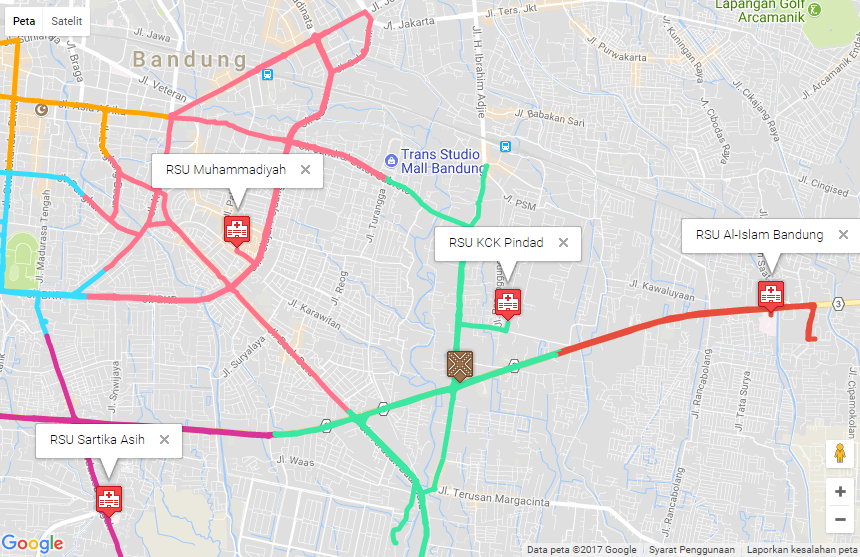
\includegraphics[scale=0.55]{data_proc_nvd_construction_2.png}
    \caption{Nearest Emergency Unit from Vertex 48}
    \label{fig:nn_vertex_48}
\end{figure}

\begin{table}[H]
\centering
\begin{tabular}{lll}
$v_{id}$       & = & 48                   \\
$v_{data}$     & = & 330 (RSU KCK Pindad) \\
$v_{distance}$ & = & 1.1390843           
\end{tabular}
\end{table}


\subsection{Determining Emergency Location}
This step is the process of determining coordinate point of emergency location. The location point of the emergency  will be the destination of the route to which selected emergency units assigned. The process of determining the location point of the incident is done by providing data in the form of latitude and longitude of the location. The location data of the emergency denote as query point (QP).

\pagebreak
For example, the determination of the location point of an emergency is shown as follows:

\begin{figure}[H]
    \centering
    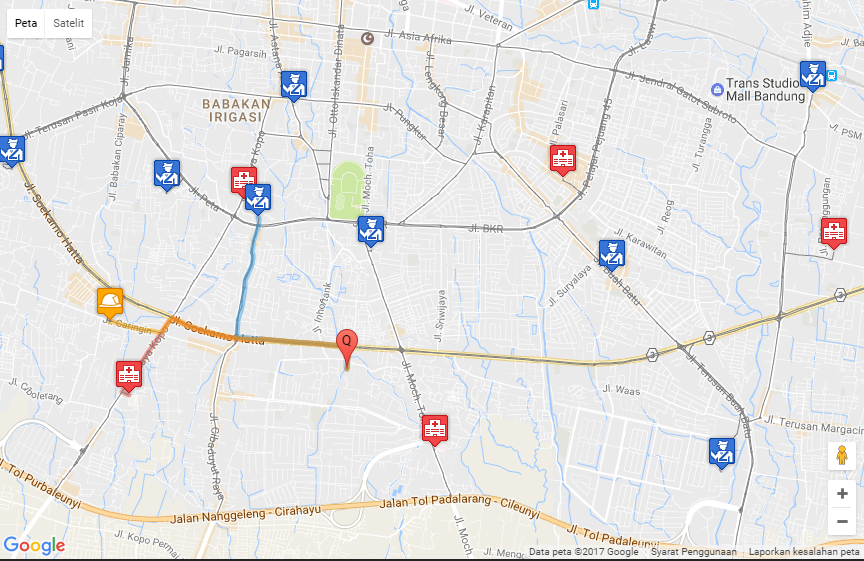
\includegraphics[scale=0.55]{data_proc_1.png}
    \caption{Emergency Location Coordinate}
    \label{fig:emergency_location_coordinate}
\end{figure}

\begin{table}[]
\centering
\begin{tabular}{lll}
Location  & = & Soekarno Hatta St. No. 396 D \\
Latitude  & = & -6.949942641719169           \\
Lomgitude & = & 107.6047620177269           
\end{tabular}
\end{table}


\subsection{Determining K-Nearest Unit to Emergency Location}
In this step, NVD-based KNN algorithms used to determining of k-nearest emergency unit. As an example of implementing the algorithm, suppose there is a query point (QP) in the form of emergency site location shown as following:

\begin{table}[H]
\centering
\begin{tabular}{lll}
Latitude   & = & -6.949942641719169 \\
Longitude  & = & 107.6047620177269  \\
Type Unit  & = & Ambulance          \\
K-Selected & = & 3                 
\end{tabular}
\end{table}

\pagebreak
NVD-based KNN algorithm requires network data voronoi diagram with k = 1 which has been done at nvd construction step. So that way, RSU Sartika Asih is the nearest emergency unit. The ambulance data inserted into the queue which sorted by the minimum distance shortest path as shown as follows:

\begin{table}[H] 
\centering
\begin{tabular}{|c|c|c|c|}
\hline
\textbf{No} & \textbf{Id} & \textbf{Name} & \textbf{Distance} \\
\hline
1 &  332 & RSU Sartika Asih & 1.6395278794745\\
\hline
\end{tabular}
\caption{Queue Initialization for Determining K-Nearest Emergency Unit}
\label{table:pq_initialization_3}
\end{table}

Furthermore, it is repeated with conditions for k obtained less or equal to the number of inputs k for this case k = 3. In each iteration $ v_ {min} $ selected by extracting emergency unit from queue which has minimum distance to emergency location (QP). Based on queue condition, the $ v_ {min} $ data obtained are as follows:

\begin{table}[H]
\centering{
\begin{tabular}{lll}
Id Generator & = & 332 \\
Name & = & RSU Sartika Asih \\
Distance & = & 1.6395278794745 \\
\end{tabular}}
\end{table}

Then, for every adjacent generator from $v_ {min}$ will be denoted as ($g_ {adj}$). Each $g_ {adj}$ inserted into queue and re-sorted queue by distance to QP. The result of inserting all $g_ {adj}$ from $v_ {min}$ is shown as follows:

\begin{table}[H] 
\centering
\begin{tabular}{|c|c|c|c|}
\hline
\textbf{No} & \textbf{Id} & \textbf{Name} & \textbf{Distance} \\
\hline
1 &  336 & RSU Immanuel & 2.531931093101\\
\hline
2 &  330 & RSU KCK Pindad & 5.4464306765158\\
\hline
\end{tabular}
\caption{PQ after Vertex 332's $g_{adj}$ inserted}
\label{table:tblhospital}
\end{table}

Then for k = 2 looping is done again. So based on queue above $v_min$ obtained as follows:

\begin{table}[H]
\centering{
\begin{tabular}{lll}
Id Generator & = & 336 \\
Name & = & RSU Immanuel \\
Distance & = & 2.531931093101 \\
\end{tabular}}
\end{table}

From the data $v_ {min}$ is done another search for $g_ {adj}$ which adjacent with $v_ {min}$. The result of inserting all $g_ {adj}$ from $v_ {min}$ is shown as follows:

\begin{table}[H] 
\centering
\begin{tabular}{|c|c|c|c|}
\hline
\textbf{No} & \textbf{Id} & \textbf{Name} & \textbf{Distance} \\
\hline
1 &  334 & RSU Immanuel & 2.6146168326924\\
\hline
2 &  338 & RSU Muhammadiyah Bandung & 4.2866445278889\\
\hline
2 &  324 & RSU Kebonjati & 4.8944211548207\\
\hline
2 &  328 & RSU Santosa Bandung Central & 4.9535388884729\\
\hline
2 &  330 & RSU KCK Pindad & 5.4464306765158\\
\hline
\end{tabular}
\caption{Hospital Data}
\label{table:tblhospital}
\end{table}

Due to the amount of looping has equal to value k which is 3, then based on queue the 3rd-nearest emergency unit shown as follows:

\begin{figure}[H]
    \centering
    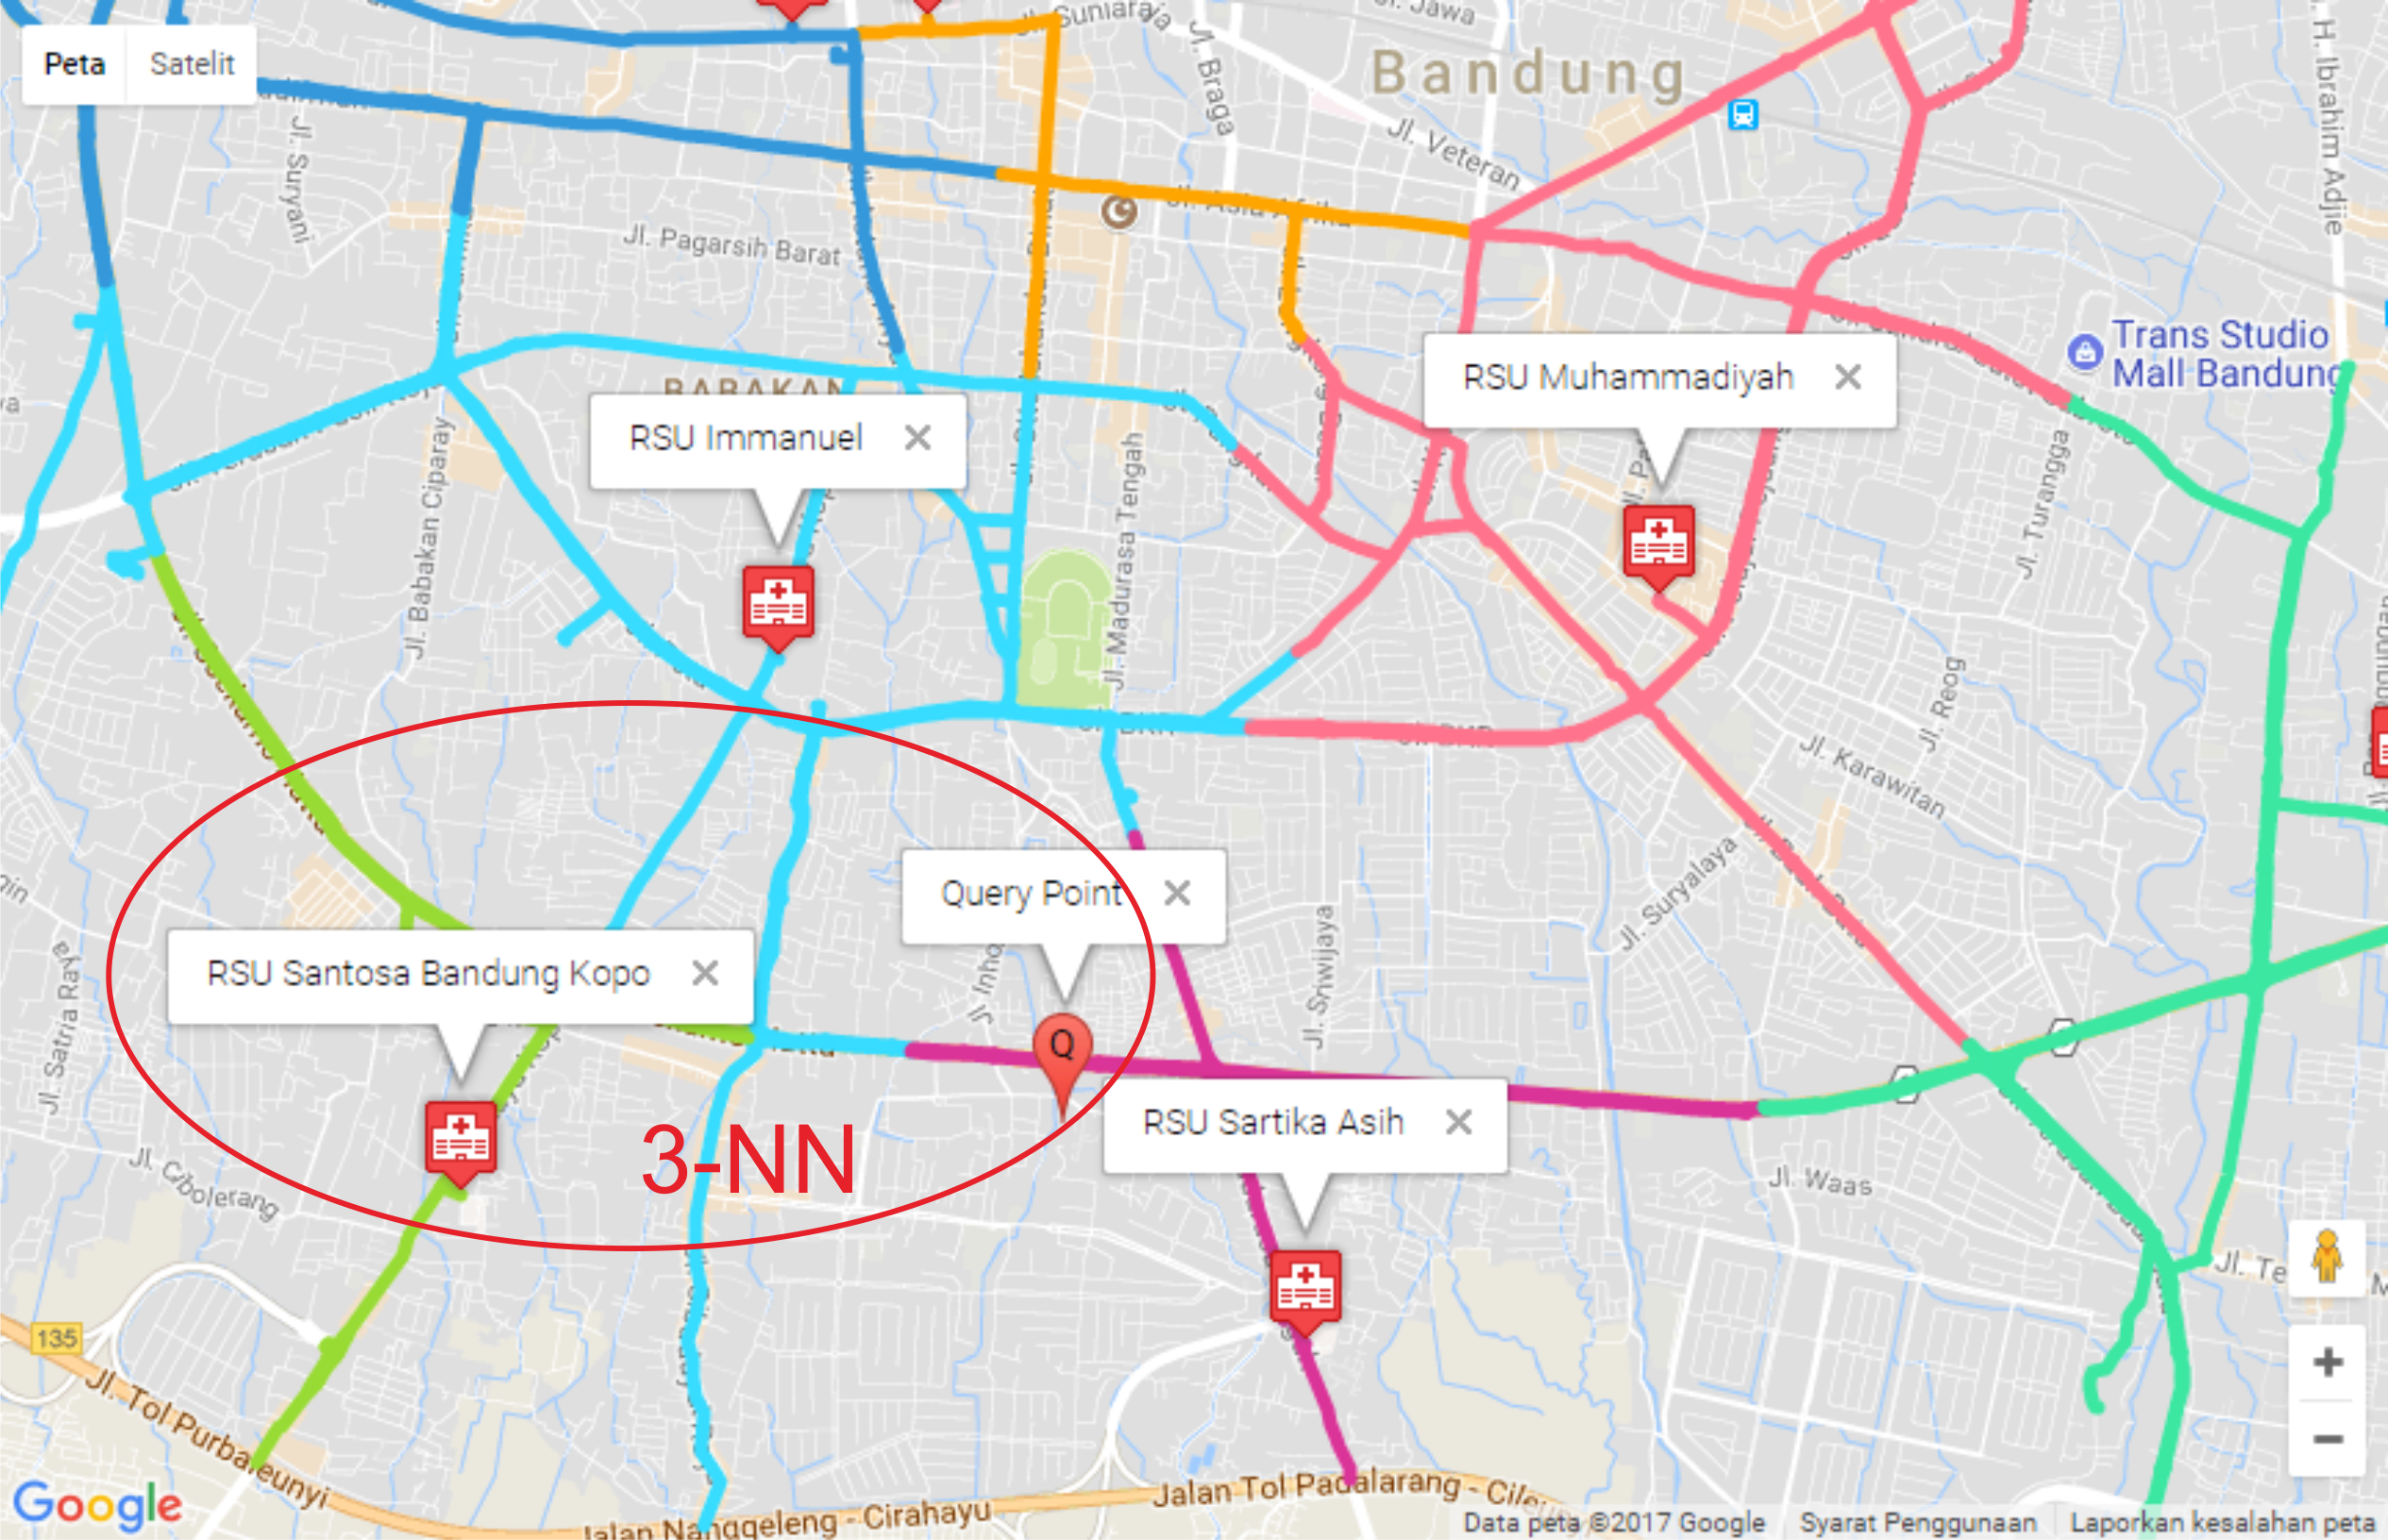
\includegraphics[scale=0.55]{data_proc_nvd-based_knn_3.png}
    \caption{3rd-Nearest Emergency Unit from QP}
    \label{fig:emergency_location_coordinate}
\end{figure}

\begin{table}[H]
\centering{
\begin{tabular}{lll}
Id Generator & = & 334 \\
Name & = & RSU Santosa Bandung Kopo \\
Latitude & = & -6.952198 \\
Longitude & = & 107.586060 \\
Type Unit & = & Ambulance \\
\end{tabular}}
\end{table}

\pagebreak
\subsection{Determining Shortest Path from Selected Emergency Unit to Emergency Location}
This step are based on the emergency location and selected units based on the previous step. The following are the data required for determining route from selected unit to emergency location:
\begin{table}[H]
\centering{
\begin{tabular}{lll}
Emergency Location & = & Jl. Soekarno Hatta \\
Latitude & = & -6.949942641719169 \\
Longitude & = & 107.6047620177269 \\
K-Selected & = & 3-NN \\
Responsible Ambulance & = & RSU Santosa Bandung Kopo \\
\end{tabular}}
\end{table}

So the shortest route from the ambulance unit responsible to the location point of the event is as follows:

\begin{figure}[H]
    \centering
    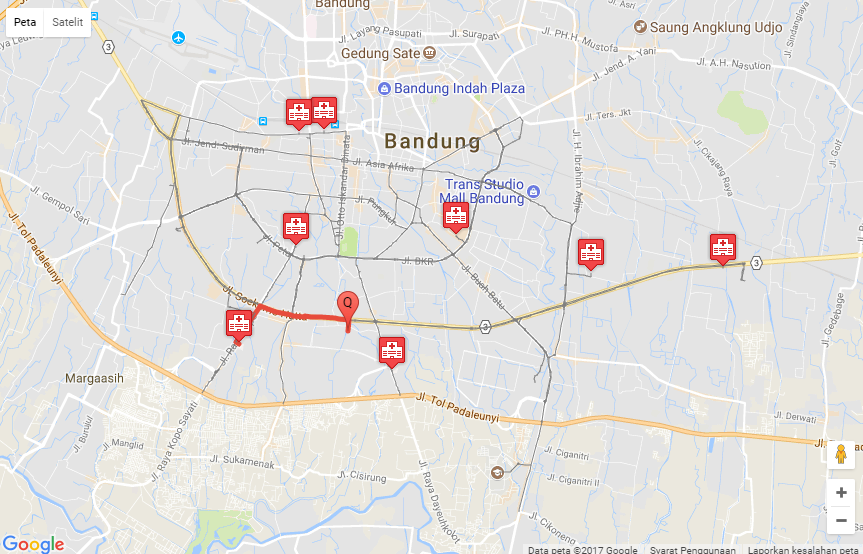
\includegraphics[scale=0.6]{rute_ambulans1.png}
    \caption{3-NN ambulance to emergency location}
    \label{fig:my_label}
\end{figure}
